%% LaTeX-Beamer template for KIT design
%% by Erik Burger, Christian Hammer
%% title picture by Klaus Krogmann
%%
%% version 2.1
%%
%% mostly compatible to KIT corporate design v2.0
%% http://intranet.kit.edu/gestaltungsrichtlinien.php
%%
%% Problems, bugs and comments to
%% burger@kit.edu

\documentclass[18pt]{beamer}
\usepackage[utf8x]{inputenc}
\usepackage{units}
\usepackage{booktabs}

%% CUSTOM
\usepackage{amsmath}
\usepackage{algpseudocode}

%% Definitions
\DeclareMathOperator{\div2}{div}
\renewcommand{\algorithmicrequire}{\textbf{Input:}}
\renewcommand{\algorithmicensure}{\textbf{Output:}}
\algnewcommand\algorithmicto{\textbf{to}}
\algrenewtext{For}[3]{\algorithmicfor\ $#1 \gets #2$ \algorithmicto\ $#3$ \algorithmicdo}
\algnewcommand\algorithmicod{\textbf{od}}
\algrenewtext{EndWhile}{\algorithmicod}
\algrenewtext{EndFor}{\algorithmicod}
%\AtBeginSection[]{%
%\begin{frame}<beamer> % do nothing in handouts
%    \frametitle{Überblick}
%    \tableofcontents[sectionstyle=show/shaded,
%    subsectionstyle=show/show/hide]
%\end{frame}
%}
%\AtBeginSubsection[]{%
%\begin{frame}<beamer> % do nothing in handouts
%    \frametitle{Überblick}
%    \tableofcontents[sectionstyle=show/shaded,
%    subsectionstyle=show/shaded/hide]
%\end{frame}
%}

%% SLIDE FORMAT

% use 'beamerthemekit' for standard 4:3 ratio
% for widescreen slides (16:9), use 'beamerthemekitwide'

\usepackage{templates/beamerthemekit}
%\usepackage{templates/beamerthemekitwide}

 %% TITLE PICTURE

 % if a custom picture is to be used on the title page, copy it into the 'logos'
 % directory, in the line below, replace 'mypicture' with the 
 % filename (without extension) and uncomment the following line
 % (picture proportions: 63 : 20 for standard, 169 : 40 for wide
 % *.eps format if you use latex+dvips+ps2pdf, 
 % *.jpg/*.png/*.pdf if you use pdflatex)


 \titleimage{banner}
 
 
%% Define some colors:
\definecolor{darkblue}{rgb}{0,0,.5}
\definecolor{darkgreen}{rgb}{0,.5,0}

 %% TITLE LOGO

 % for a custom logo on the front page, copy your file into the 'logos'
 % directory, insert the filename in the line below and uncomment it

\titlelogo{logo_150x150}
 
 % (*.eps format if you use latex+dvips+ps2pdf,
 % *.jpg/*.png/*.pdf if you use pdflatex)
 
 %% TikZ INTEGRATION
 
 % use these packages for PCM symbols and UML classes
 % \usepackage{templates/tikzkit}
 % \usepackage{templates/tikzuml}
 
 % the presentation starts here
 
\author{Dominik Muth - dominik.muth@student.kit.edu}
\institute{Institut f\"ur Informatik}


\title[Tutorium 13]{GBI Tutorium Nr. $2^5$}
\subtitle{Tutorium 13}
\date{30. Januar 2013}

% Bibliography



\begin{document}

	%title page
	\begin{frame}
		\titlepage
	\end{frame}

	%table of contents
	\begin{frame}{Outline/Gliederung}
		\tableofcontents
	\end{frame}	
		
	
	
	\section{Wiederholung} 
	\begin{frame} {Wiederholung - Quiz}
		\begin{itemize}
			
			\item Rechtslineare Grammatiken lassen sich durch Automaten darstellen.
			\only<2-> {\color{darkgreen}$\surd$}\\
			\color{black}
			\item $T(n)=8T(\frac{n}{2})+1000n^2 \in \Theta(n^4)$
			\only<3-> {\color{red}$X$}\\
			\color{black}
			
			\item Mit Touringmaschinen lassen sich alle Probleme lösen.
			\only<4-> {\color{red}$X$}\\
			\color{black}
	
			\item Mit Touringmaschinen kann man Touringmaschinen simulieren.
			\only<5-> {\color{darkgreen}$\surd$}\\
			\color{black}
		\end{itemize}
	\end{frame}
	
	
	\begin{frame}{Wiederholung - Induktion}
		\begin{block}{Übungsblatt 10- Aufgabe 10.2}
			Gegeben sei folgende Funktion $T(n)$, für $n \in \mathbb{N}_+$:\\
			\[T(1) = 0 \text{, \hspace{20pt}} \forall n > 2; T(n) = \sqrt{n} \cdot T(\lfloor \sqrt{n} \rfloor ) + n\]\\
			\begin{itemize}
				\item Zeigen Sie durch vollständige Induktion: $T(n) \in \mathcal{O}(n\: log_2(log_2(n))$
			\end{itemize}
		\end{block}
	\end{frame}
	
	
	\section{Fragen}
	\begin{frame} {Fragen}
		\begin{itemize}
			\item Fragen zum Stoff?
			\item Fragen zum n\"achsten \"Ubungsblatt?
			\item Generelle Fragen?
			\item Feedback?
		\end{itemize}
	\end{frame}	
	
	
	
	\section{Unentscheidbare Probleme}
	\begin{frame}{Unentscheidbare Probleme}
		\begin{block}{Entscheidbar}
			\pause
			Für ein entscheidbares Problem gibt es eine Turingmaschine, 
			welche für jede Eingabe hält und das Eingabewort entweder akzeptiert oder nicht.
		\end{block}
			\pause
		\begin{block}{Unentscheidbar}
			\visible<4->{
				Für ein unentscheidbares Problem existiert keine Turingmaschine, 
				welche für jede Eingabe hält und das Eingabewort entweder akzeptiert oder nicht.
			}
		\end{block}
	\end{frame}
	
	
	\begin{frame}{Unentscheidbare Probleme}
		\begin{exampleblock}{Beispiel}
			\begin{algorithmic}
				\State $n \gets Eingabe$
				\While{$n > 1$}
					\If{$n\: mod \:2 = 0$}
						\State $n \gets n/2$
					\Else
						\State $n \gets 3n + 1$
					\EndIf
				\EndWhile
			\end{algorithmic}
		\end{exampleblock}
	\end{frame}
	
	
	\section{Äquivalenzrelationen}
	\begin{frame}{Äquivalenzrelationen}
		\begin{block}{Wie war eine Äquivalenzrelation definiert?}
			Eine Relation R ist genau dann eine \textbf{Äquivalenzrelation}, wenn sie
			\begin{itemize}
				\item $ $ \visible<2->{symmetrisch,}
				\item $ $ \visible<3->{reflexiv und}
				\item $ $ \visible<4->{transitiv}
			\end{itemize}
			ist.
		\end{block}
	\end{frame}
	
	\begin{frame}{Äquivalenzrelationen}
		Welche Eigenschaften haben folgende Relationen ($\mathbb{Z} \rightarrow \mathbb{Z}$)
		\begin{itemize}
			\item $\leq$ \visible<2->{reflexiv, transitiv}
			\item $>$ \visible<3->{transitiv}
			\item $=$ \visible<4->{reflexiv, transitiv, symmetrisch}
		\end{itemize}
		
		\visible<5->{Wie sehen die Relationen in einem Graphen aus?}
	\end{frame}
	
	\begin{frame}{Äquivalenzklassen}
		\begin{block}{Definition}
			Sind zwei Elemente $(x,y) \in R$, so schreit man auch $xRy$ (Infixschreibweise).\\
			Alle Element, welche miteinander in Relation stehen (vorausgesetzt R ist eine Äquivalenzrelation, auf der Menge $M$), befinden sich in der selben Äquivalenzklasse.\\
			Wir schreiben dann:\\
			\[ [y]_R = \{x\in M\;|\; xRy\}\] 
		\end{block}
	\end{frame}
	
	\begin{frame}{Nerode-Äquivalenz}
		\begin{block}{Definition}
			Zwei Wörter sind bezüglich der Nerode-Relation($\equiv_L$) genau dann äquivalent zueinander, wenn sie beide durch exakt dieselben Suffixe zu Wörtern der Sprache L ergänzt werden.\\
		\end{block}
		
		\begin{exampleblock}{Beispiel}
			Sei $A = {0,1}$ und $L = \langle 0*1* \rangle$\\
			\vspace{10pt}
			Es gibt also exakt 3 Nerode Äquivalenzklassen für die gegebene Sprache:\\
			\begin{itemize}
				\item Die Äquivalenzklasse $[0]$ enthält alle Wörter ohne eine 1: $\{0\}^*$
				\item Die Äquivalenzklasse $[1]$ enthält alle Wörter mit min. einer 1 am Ende:
				 $\{0\}^*\{1\}^+$
				\item Die Äquivalenzklasse $[10]$ enthält alle ungültigen Wörter:
				$\{0,1\}^*\{10\}\{0,1\}^*$
			\end{itemize}
		
		\end{exampleblock}
	\end{frame}
		
		
	\begin{frame}{Quiz}
		\begin{itemize}
			\item $xRy \Rightarrow [x]_R = [y]_R$
				\visible<2->{\color{darkgreen}$\surd$}\\
			\color{black}
			\item $\exists z \in M\;|\;z\in [x]_R \land z \in [y]_R \Rightarrow [x]_R = [y]_R$
				\visible<3->{\color{darkgreen}$\surd$}\\
			\color{black}
			\item Wie viele Äquivalenzklassen gibt es zu $R =  \mathbb{N} \rightarrow \mathbb{N}: y = x\: mod\: 6$?
				\visible<4->{\color{red}Keine, R ist keine Äquivalenzrelation!}\\ 
				\vspace{10pt}
				\visible<5->{\color{black}Wie muss man R ändern, 
				damit es eine Äquivalenzrelation ist, 
				und wie viele Äquivalenzklassen hat sie dann?}\\
				\visible<6->{\color{darkgreen}
				$R_2 =  \mathbb{N} \rightarrow \mathbb{N}: y\: mod\: 6 = x\: mod\: 6$\\
				Die Äquivalenzrelation $R_2$ hat 6 Äquivalenzklassen }
		\end{itemize}
	\end{frame}
	
	
	
	\section{Klausuraufgaben}
	\begin{frame}{Klausuraufgabe}
		\begin{block}{Sommer Semester 2010 - Aufgabe 2 (3 + 2 Punkte)}
		\begin{itemize}
				\item Gegeben sei die Formel \\
				$F = (A\Rightarrow B) \Rightarrow ((B \Rightarrow A) \Rightarrow B)$.\\
				Stellen sie eine Wahrheitstabelle für 
				$F$ auf und geben sie eine äquivalente Formel
				$F'$ an, welche sowohl A als auch B maximal ein mal enthält, und $F = F'$ gilt.
			
				\item Gegeben seien die Formeln:\\
					$F_1 = (((B \Rightarrow A) \lor B) \Rightarrow (\neg A)) \land B$\\
					und\\
					$F_2 = \neg A \land B$\\
					Zeigen Sie (zum Beispiel mit Wahrheitstabellen), 
					dass $F_1$ und $F_2$ äquivalent sind.
			\end{itemize}
		\end{block}
	\end{frame}
	
	
	\begin{frame}{Klausuraufgabe}
		\begin{block}{Sommer Semester 2010 - Aufgabe 3 (6 Punkte)}
			\small
			Gegeben seien $3^n$ Kugeln, von denen eine Kugel 1,01 kg wiegt und alle anderen
			Kugeln 1 kg wiegen, und die ansonsten nicht zu unterscheiden sind.
			Man hat eine Waage, 
			mit der man die Gewichte zweier beliebig großer Mengen von Kugeln vergleichen kann:
			\begin{itemize}
				\item Falls das Gewicht in beiden verglichenen Mengen gleich ist,
				gibt die Waage den Wert 0 zurück.
				
				\item Falls das Gewicht in der linken Waagschale größer als das Gewicht in der 
				rechten Waagschale ist, gibt die Waage den Wert 1 zurück.
						
				\item Falls das Gewicht in der linken Waagschale kleiner als das
				Gewicht in der rechten Waagschale ist, gibt die Waage den Wert -1 zurück.
			\end{itemize}

			Zeigen Sie durch vollständige Induktion über n :\\
			Man kann durch n-maliges Vergleichen mit der Waage die Kugel K herausfinden, 
			die 1,01 kg wiegt.
		\end{block}
	\end{frame}
		
	\begin{frame} {EOF}
		\begin{center}
			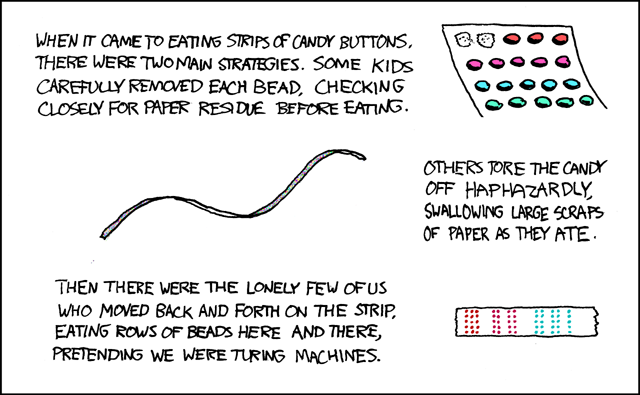
\includegraphics[scale=0.45]{graphics/eof13.png}\\
			\tiny $source: http://imgs.xkcd.com/comics/candy\_button\_paper.png$
		\end{center}
	\end{frame}

\end{document}
